% Created by tikzDevice version 0.12 on 2019-06-13 17:21:57
% !TEX encoding = UTF-8 Unicode
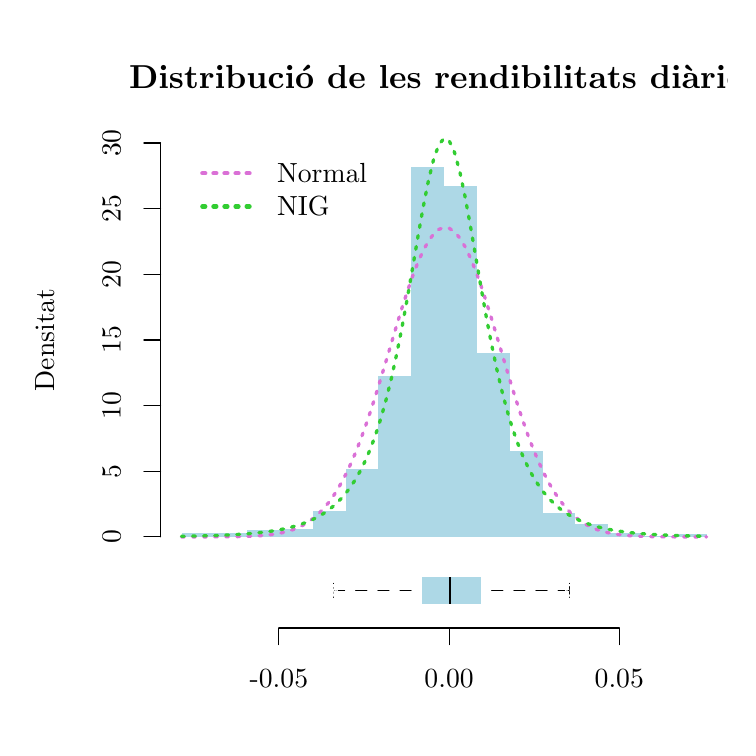
\begin{tikzpicture}[x=1pt,y=1pt]
\definecolor{fillColor}{RGB}{255,255,255}
\path[use as bounding box,fill=fillColor,fill opacity=0.00] (0,0) rectangle (252.94,252.94);
\begin{scope}
\path[clip] ( 48.00, 36.00) rectangle (252.94, 63.24);
\definecolor{fillColor}{RGB}{173,216,230}

\path[fill=fillColor] (142.38, 44.57) --
	(142.38, 54.66) --
	(163.94, 54.66) --
	(163.94, 44.57) --
	cycle;
\definecolor{drawColor}{RGB}{0,0,0}

\path[draw=drawColor,line width= 0.4pt,line join=round] (152.60, 44.57) -- (152.60, 54.66);

\path[draw=drawColor,line width= 0.4pt,dash pattern=on 4pt off 4pt ,line join=round,line cap=round] (110.55, 49.62) -- (142.38, 49.62);

\path[draw=drawColor,line width= 0.4pt,dash pattern=on 4pt off 4pt ,line join=round,line cap=round] (195.67, 49.62) -- (163.94, 49.62);

\path[draw=drawColor,line width= 0.4pt,line join=round,line cap=round] (110.55, 47.10) -- (110.55, 52.14);

\path[draw=drawColor,line width= 0.4pt,line join=round,line cap=round] (195.67, 47.10) -- (195.67, 52.14);
\definecolor{drawColor}{RGB}{255,255,255}

\path[draw=drawColor,line width= 0.4pt,line join=round,line cap=round] (142.38, 44.57) --
	(142.38, 54.66) --
	(163.94, 54.66) --
	(163.94, 44.57) --
	(142.38, 44.57);

\path[draw=drawColor,line width= 0.4pt,line join=round,line cap=round] ( 85.57, 49.62) circle (  2.25);

\path[draw=drawColor,line width= 0.4pt,line join=round,line cap=round] ( 60.58, 49.62) circle (  2.25);

\path[draw=drawColor,line width= 0.4pt,line join=round,line cap=round] (198.27, 49.62) circle (  2.25);

\path[draw=drawColor,line width= 0.4pt,line join=round,line cap=round] (196.62, 49.62) circle (  2.25);

\path[draw=drawColor,line width= 0.4pt,line join=round,line cap=round] (107.04, 49.62) circle (  2.25);

\path[draw=drawColor,line width= 0.4pt,line join=round,line cap=round] (197.12, 49.62) circle (  2.25);

\path[draw=drawColor,line width= 0.4pt,line join=round,line cap=round] ( 72.66, 49.62) circle (  2.25);

\path[draw=drawColor,line width= 0.4pt,line join=round,line cap=round] (215.76, 49.62) circle (  2.25);

\path[draw=drawColor,line width= 0.4pt,line join=round,line cap=round] ( 95.39, 49.62) circle (  2.25);

\path[draw=drawColor,line width= 0.4pt,line join=round,line cap=round] ( 99.96, 49.62) circle (  2.25);

\path[draw=drawColor,line width= 0.4pt,line join=round,line cap=round] (210.64, 49.62) circle (  2.25);

\path[draw=drawColor,line width= 0.4pt,line join=round,line cap=round] (109.18, 49.62) circle (  2.25);

\path[draw=drawColor,line width= 0.4pt,line join=round,line cap=round] (103.93, 49.62) circle (  2.25);

\path[draw=drawColor,line width= 0.4pt,line join=round,line cap=round] ( 88.74, 49.62) circle (  2.25);

\path[draw=drawColor,line width= 0.4pt,line join=round,line cap=round] (209.15, 49.62) circle (  2.25);

\path[draw=drawColor,line width= 0.4pt,line join=round,line cap=round] (203.89, 49.62) circle (  2.25);

\path[draw=drawColor,line width= 0.4pt,line join=round,line cap=round] (203.49, 49.62) circle (  2.25);

\path[draw=drawColor,line width= 0.4pt,line join=round,line cap=round] (101.22, 49.62) circle (  2.25);

\path[draw=drawColor,line width= 0.4pt,line join=round,line cap=round] (200.30, 49.62) circle (  2.25);

\path[draw=drawColor,line width= 0.4pt,line join=round,line cap=round] (108.24, 49.62) circle (  2.25);

\path[draw=drawColor,line width= 0.4pt,line join=round,line cap=round] ( 67.83, 49.62) circle (  2.25);

\path[draw=drawColor,line width= 0.4pt,line join=round,line cap=round] (214.16, 49.62) circle (  2.25);

\path[draw=drawColor,line width= 0.4pt,line join=round,line cap=round] (206.14, 49.62) circle (  2.25);

\path[draw=drawColor,line width= 0.4pt,line join=round,line cap=round] (243.51, 49.62) circle (  2.25);

\path[draw=drawColor,line width= 0.4pt,line join=round,line cap=round] ( 98.46, 49.62) circle (  2.25);

\path[draw=drawColor,line width= 0.4pt,line join=round,line cap=round] (245.35, 49.62) circle (  2.25);

\path[draw=drawColor,line width= 0.4pt,line join=round,line cap=round] (222.55, 49.62) circle (  2.25);

\path[draw=drawColor,line width= 0.4pt,line join=round,line cap=round] (212.08, 49.62) circle (  2.25);

\path[draw=drawColor,line width= 0.4pt,line join=round,line cap=round] (101.17, 49.62) circle (  2.25);

\path[draw=drawColor,line width= 0.4pt,line join=round,line cap=round] ( 83.86, 49.62) circle (  2.25);

\path[draw=drawColor,line width= 0.4pt,line join=round,line cap=round] (100.64, 49.62) circle (  2.25);

\path[draw=drawColor,line width= 0.4pt,line join=round,line cap=round] ( 79.93, 49.62) circle (  2.25);

\path[draw=drawColor,line width= 0.4pt,line join=round,line cap=round] (108.84, 49.62) circle (  2.25);

\path[draw=drawColor,line width= 0.4pt,line join=round,line cap=round] ( 73.53, 49.62) circle (  2.25);

\path[draw=drawColor,line width= 0.4pt,line join=round,line cap=round] (106.94, 49.62) circle (  2.25);

\path[draw=drawColor,line width= 0.4pt,line join=round,line cap=round] (201.77, 49.62) circle (  2.25);

\path[draw=drawColor,line width= 0.4pt,line join=round,line cap=round] (106.44, 49.62) circle (  2.25);

\path[draw=drawColor,line width= 0.4pt,line join=round,line cap=round] (104.11, 49.62) circle (  2.25);

\path[draw=drawColor,line width= 0.4pt,line join=round,line cap=round] (103.10, 49.62) circle (  2.25);

\path[draw=drawColor,line width= 0.4pt,line join=round,line cap=round] ( 55.59, 49.62) circle (  2.25);

\path[draw=drawColor,line width= 0.4pt,line join=round,line cap=round] ( 81.64, 49.62) circle (  2.25);

\path[draw=drawColor,line width= 0.4pt,line join=round,line cap=round] (205.97, 49.62) circle (  2.25);

\path[draw=drawColor,line width= 0.4pt,line join=round,line cap=round] (109.61, 49.62) circle (  2.25);

\path[draw=drawColor,line width= 0.4pt,line join=round,line cap=round] (211.73, 49.62) circle (  2.25);

\path[draw=drawColor,line width= 0.4pt,line join=round,line cap=round] (202.61, 49.62) circle (  2.25);

\path[draw=drawColor,line width= 0.4pt,line join=round,line cap=round] ( 63.93, 49.62) circle (  2.25);

\path[draw=drawColor,line width= 0.4pt,line join=round,line cap=round] (105.20, 49.62) circle (  2.25);

\path[draw=drawColor,line width= 0.4pt,line join=round,line cap=round] (231.79, 49.62) circle (  2.25);
\end{scope}
\begin{scope}
\path[clip] (  0.00,  0.00) rectangle (252.94,252.94);
\definecolor{drawColor}{RGB}{0,0,0}

\path[draw=drawColor,line width= 0.4pt,line join=round,line cap=round] ( 90.78, 36.00) -- (213.78, 36.00);

\path[draw=drawColor,line width= 0.4pt,line join=round,line cap=round] ( 90.78, 36.00) -- ( 90.78, 30.00);

\path[draw=drawColor,line width= 0.4pt,line join=round,line cap=round] (152.28, 36.00) -- (152.28, 30.00);

\path[draw=drawColor,line width= 0.4pt,line join=round,line cap=round] (213.78, 36.00) -- (213.78, 30.00);

\node[text=drawColor,anchor=base,inner sep=0pt, outer sep=0pt, scale=  1.00] at ( 90.78, 14.40) {-0.05};

\node[text=drawColor,anchor=base,inner sep=0pt, outer sep=0pt, scale=  1.00] at (152.28, 14.40) {0.00};

\node[text=drawColor,anchor=base,inner sep=0pt, outer sep=0pt, scale=  1.00] at (213.78, 14.40) {0.05};
\end{scope}
\begin{scope}
\path[clip] (  0.00, 63.24) rectangle (252.94,252.94);
\definecolor{drawColor}{RGB}{0,0,0}

\node[text=drawColor,anchor=base,inner sep=0pt, outer sep=0pt, scale=  1.20] at (150.47,230.80) {\bfseries Distribució de les rendibilitats diàries};

\node[text=drawColor,rotate= 90.00,anchor=base,inner sep=0pt, outer sep=0pt, scale=  1.00] at (  9.60,140.09) {Densitat};
\end{scope}
\begin{scope}
\path[clip] (  0.00,  0.00) rectangle (252.94,252.94);
\definecolor{drawColor}{RGB}{0,0,0}

\path[draw=drawColor,line width= 0.4pt,line join=round,line cap=round] ( 48.00, 68.93) -- ( 48.00,211.25);

\path[draw=drawColor,line width= 0.4pt,line join=round,line cap=round] ( 48.00, 68.93) -- ( 42.00, 68.93);

\path[draw=drawColor,line width= 0.4pt,line join=round,line cap=round] ( 48.00, 92.65) -- ( 42.00, 92.65);

\path[draw=drawColor,line width= 0.4pt,line join=round,line cap=round] ( 48.00,116.37) -- ( 42.00,116.37);

\path[draw=drawColor,line width= 0.4pt,line join=round,line cap=round] ( 48.00,140.09) -- ( 42.00,140.09);

\path[draw=drawColor,line width= 0.4pt,line join=round,line cap=round] ( 48.00,163.81) -- ( 42.00,163.81);

\path[draw=drawColor,line width= 0.4pt,line join=round,line cap=round] ( 48.00,187.53) -- ( 42.00,187.53);

\path[draw=drawColor,line width= 0.4pt,line join=round,line cap=round] ( 48.00,211.25) -- ( 42.00,211.25);

\node[text=drawColor,rotate= 90.00,anchor=base,inner sep=0pt, outer sep=0pt, scale=  1.00] at ( 33.60, 68.93) {0};

\node[text=drawColor,rotate= 90.00,anchor=base,inner sep=0pt, outer sep=0pt, scale=  1.00] at ( 33.60, 92.65) {5};

\node[text=drawColor,rotate= 90.00,anchor=base,inner sep=0pt, outer sep=0pt, scale=  1.00] at ( 33.60,116.37) {10};

\node[text=drawColor,rotate= 90.00,anchor=base,inner sep=0pt, outer sep=0pt, scale=  1.00] at ( 33.60,140.09) {15};

\node[text=drawColor,rotate= 90.00,anchor=base,inner sep=0pt, outer sep=0pt, scale=  1.00] at ( 33.60,163.81) {20};

\node[text=drawColor,rotate= 90.00,anchor=base,inner sep=0pt, outer sep=0pt, scale=  1.00] at ( 33.60,187.53) {25};

\node[text=drawColor,rotate= 90.00,anchor=base,inner sep=0pt, outer sep=0pt, scale=  1.00] at ( 33.60,211.25) {30};
\end{scope}
\begin{scope}
\path[clip] ( 48.00, 63.24) rectangle (252.94,216.94);
\definecolor{fillColor}{RGB}{173,216,230}

\path[fill=fillColor] ( 55.59, 68.93) rectangle ( 67.45, 70.35);

\path[fill=fillColor] ( 67.45, 68.93) rectangle ( 79.31, 70.35);

\path[fill=fillColor] ( 79.31, 68.93) rectangle ( 91.17, 71.29);

\path[fill=fillColor] ( 91.17, 68.93) rectangle (103.03, 71.76);

\path[fill=fillColor] (103.03, 68.93) rectangle (114.89, 78.38);

\path[fill=fillColor] (114.89, 68.93) rectangle (126.75, 93.50);

\path[fill=fillColor] (126.75, 68.93) rectangle (138.61,127.05);

\path[fill=fillColor] (138.61, 68.93) rectangle (150.47,202.65);

\path[fill=fillColor] (150.47, 68.93) rectangle (162.33,195.56);

\path[fill=fillColor] (162.33, 68.93) rectangle (174.19,135.55);

\path[fill=fillColor] (174.19, 68.93) rectangle (186.05,100.12);

\path[fill=fillColor] (186.05, 68.93) rectangle (197.91, 77.43);

\path[fill=fillColor] (197.91, 68.93) rectangle (209.77, 73.65);

\path[fill=fillColor] (209.77, 68.93) rectangle (221.63, 70.35);

\path[fill=fillColor] (221.63, 68.93) rectangle (233.49, 69.40);

\path[fill=fillColor] (233.49, 68.93) rectangle (245.35, 69.87);
\definecolor{drawColor}{RGB}{218,112,214}

\path[draw=drawColor,line width= 1.2pt,dash pattern=on 1pt off 3pt ,line join=round,line cap=round] ( 55.59, 68.93) --
	( 57.49, 68.93) --
	( 59.39, 68.93) --
	( 61.28, 68.93) --
	( 63.18, 68.94) --
	( 65.08, 68.94) --
	( 66.98, 68.95) --
	( 68.87, 68.96) --
	( 70.77, 68.97) --
	( 72.67, 68.99) --
	( 74.57, 69.01) --
	( 76.46, 69.05) --
	( 78.36, 69.09) --
	( 80.26, 69.16) --
	( 82.16, 69.25) --
	( 84.06, 69.37) --
	( 85.95, 69.53) --
	( 87.85, 69.74) --
	( 89.75, 70.02) --
	( 91.65, 70.38) --
	( 93.54, 70.83) --
	( 95.44, 71.41) --
	( 97.34, 72.13) --
	( 99.24, 73.03) --
	(101.13, 74.14) --
	(103.03, 75.49) --
	(104.93, 77.11) --
	(106.83, 79.03) --
	(108.72, 81.31) --
	(110.62, 83.95) --
	(112.52, 87.01) --
	(114.42, 90.48) --
	(116.31, 94.40) --
	(118.21, 98.77) --
	(120.11,103.57) --
	(122.01,108.79) --
	(123.91,114.38) --
	(125.80,120.30) --
	(127.70,126.47) --
	(129.60,132.81) --
	(131.50,139.21) --
	(133.39,145.57) --
	(135.29,151.77) --
	(137.19,157.66) --
	(139.09,163.13) --
	(140.98,168.05) --
	(142.88,172.30) --
	(144.78,175.77) --
	(146.68,178.37) --
	(148.57,180.04) --
	(150.47,180.73) --
	(152.37,180.43) --
	(154.27,179.14) --
	(156.17,176.89) --
	(158.06,173.75) --
	(159.96,169.79) --
	(161.86,165.12) --
	(163.76,159.85) --
	(165.65,154.10) --
	(167.55,148.01) --
	(169.45,141.70) --
	(171.35,135.30) --
	(173.24,128.92) --
	(175.14,122.67) --
	(177.04,116.65) --
	(178.94,110.92) --
	(180.83,105.55) --
	(182.73,100.59) --
	(184.63, 96.05) --
	(186.53, 91.96) --
	(188.43, 88.31) --
	(190.32, 85.09) --
	(192.22, 82.29) --
	(194.12, 79.88) --
	(196.02, 77.82) --
	(197.91, 76.08) --
	(199.81, 74.63) --
	(201.71, 73.44) --
	(203.61, 72.46) --
	(205.50, 71.67) --
	(207.40, 71.04) --
	(209.30, 70.54) --
	(211.20, 70.15) --
	(213.09, 69.84) --
	(214.99, 69.61) --
	(216.89, 69.43) --
	(218.79, 69.29) --
	(220.69, 69.19) --
	(222.58, 69.12) --
	(224.48, 69.06) --
	(226.38, 69.02) --
	(228.28, 68.99) --
	(230.17, 68.97) --
	(232.07, 68.96) --
	(233.97, 68.95) --
	(235.87, 68.94) --
	(237.76, 68.94) --
	(239.66, 68.94) --
	(241.56, 68.93) --
	(243.46, 68.93) --
	(245.35, 68.93);
\definecolor{drawColor}{RGB}{50,205,50}

\path[draw=drawColor,line width= 1.2pt,dash pattern=on 1pt off 3pt ,line join=round,line cap=round] ( 55.59, 69.16) --
	( 57.49, 69.19) --
	( 59.39, 69.22) --
	( 61.28, 69.26) --
	( 63.18, 69.30) --
	( 65.08, 69.35) --
	( 66.98, 69.41) --
	( 68.87, 69.48) --
	( 70.77, 69.55) --
	( 72.67, 69.64) --
	( 74.57, 69.74) --
	( 76.46, 69.85) --
	( 78.36, 69.98) --
	( 80.26, 70.13) --
	( 82.16, 70.31) --
	( 84.06, 70.50) --
	( 85.95, 70.73) --
	( 87.85, 70.99) --
	( 89.75, 71.29) --
	( 91.65, 71.64) --
	( 93.54, 72.04) --
	( 95.44, 72.51) --
	( 97.34, 73.04) --
	( 99.24, 73.67) --
	(101.13, 74.39) --
	(103.03, 75.22) --
	(104.93, 76.20) --
	(106.83, 77.33) --
	(108.72, 78.64) --
	(110.62, 80.18) --
	(112.52, 81.97) --
	(114.42, 84.05) --
	(116.31, 86.48) --
	(118.21, 89.32) --
	(120.11, 92.62) --
	(122.01, 96.46) --
	(123.91,100.92) --
	(125.80,106.08) --
	(127.70,112.03) --
	(129.60,118.84) --
	(131.50,126.57) --
	(133.39,135.24) --
	(135.29,144.82) --
	(137.19,155.19) --
	(139.09,166.10) --
	(140.98,177.18) --
	(142.88,187.87) --
	(144.78,197.51) --
	(146.68,205.35) --
	(148.57,210.68) --
	(150.47,212.96) --
	(152.37,211.95) --
	(154.27,207.76) --
	(156.17,200.82) --
	(158.06,191.79) --
	(159.96,181.42) --
	(161.86,170.42) --
	(163.76,159.39) --
	(165.65,148.78) --
	(167.55,138.87) --
	(169.45,129.83) --
	(171.35,121.74) --
	(173.24,114.57) --
	(175.14,108.30) --
	(177.04,102.84) --
	(178.94, 98.12) --
	(180.83, 94.04) --
	(182.73, 90.54) --
	(184.63, 87.53) --
	(186.53, 84.95) --
	(188.43, 82.74) --
	(190.32, 80.84) --
	(192.22, 79.21) --
	(194.12, 77.82) --
	(196.02, 76.62) --
	(197.91, 75.59) --
	(199.81, 74.70) --
	(201.71, 73.93) --
	(203.61, 73.27) --
	(205.50, 72.71) --
	(207.40, 72.21) --
	(209.30, 71.79) --
	(211.20, 71.42) --
	(213.09, 71.10) --
	(214.99, 70.83) --
	(216.89, 70.59) --
	(218.79, 70.38) --
	(220.69, 70.20) --
	(222.58, 70.04) --
	(224.48, 69.90) --
	(226.38, 69.78) --
	(228.28, 69.68) --
	(230.17, 69.59) --
	(232.07, 69.51) --
	(233.97, 69.44) --
	(235.87, 69.38) --
	(237.76, 69.32) --
	(239.66, 69.28) --
	(241.56, 69.23) --
	(243.46, 69.20) --
	(245.35, 69.17);

\path[] ( 54.15,212.33) rectangle (127.17,176.33);
\definecolor{drawColor}{RGB}{218,112,214}

\path[draw=drawColor,line width= 1.6pt,dash pattern=on 1pt off 3pt ,line join=round,line cap=round] ( 63.15,200.33) -- ( 81.15,200.33);
\definecolor{drawColor}{RGB}{50,205,50}

\path[draw=drawColor,line width= 1.6pt,dash pattern=on 1pt off 3pt ,line join=round,line cap=round] ( 63.15,188.33) -- ( 81.15,188.33);
\definecolor{drawColor}{RGB}{0,0,0}

\node[text=drawColor,anchor=base west,inner sep=0pt, outer sep=0pt, scale=  1.00] at ( 90.15,196.89) {Normal};

\node[text=drawColor,anchor=base west,inner sep=0pt, outer sep=0pt, scale=  1.00] at ( 90.15,184.89) {NIG};
\end{scope}
\end{tikzpicture}
